\section{System Behavior}
\label{sec:SysBehavior}

The architecture description provided in this section describes the flow of the different menus for the game once started.

\begin{figure}[h]
    \centering
    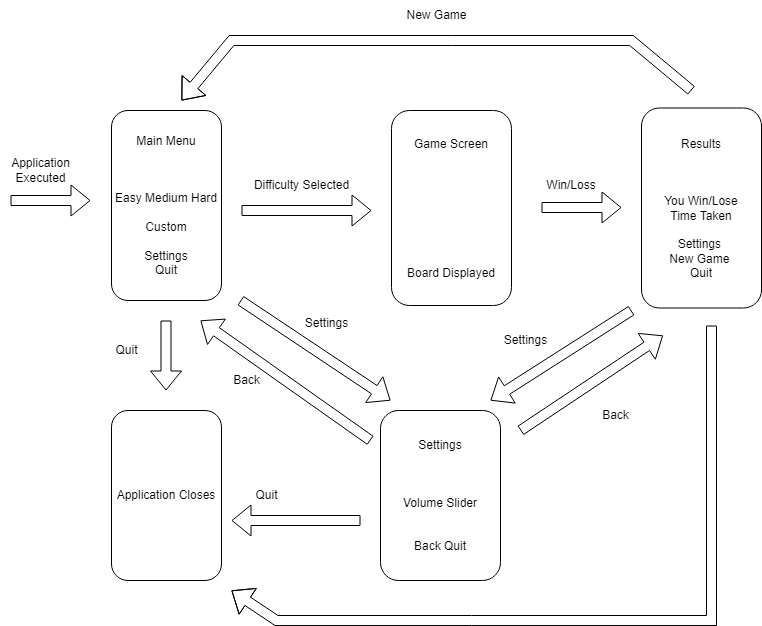
\includegraphics[width=10cm]{Images/SysBehavior.png}
       \caption{State Diagram describing the System Behavior.}
           \label{Fig:SysBehavior}
\end{figure}

As seen in Figure \ref{Fig:SysBehavior}, the game begins when the .exe file is executed.
The user is then presented with the Main Menu which allows for the user to choose a difficulty, as well as switch to the settings menu, and also to the quit the game.
From the Settings menu, a volume slider is displayed, and the user is able to go back to the previous page, either the Main Menu or the Post-Game Menu AKA Results Menu.
Should the user have selected a difficulty, then the Game Screen appears with the board with given dimensions based on the difficulty selected.
After the user has won or lost the game, the Post-Game Menu appears with a display of the time taken, a message indicating the result of the game: win/loss, a button to the Settings menu, a button connecting to the Main Menu, and a Quit button.
When the Quit button is pressed, the game closes.